\chapter{\babTiga}

% Tahapan Penelitian {{{ %
\section{Tahapan Penelitian}

Penelitian ini dilakukan melalui beberapa tahapan. Tahap yang pertama
adalah studi literatur untuk mempelajari dan memahami materi-materi terkait
dengan penelitian, seperti \tracking~serta arsitektur \pubsub. Tahapan yang
kedua yaitu melakukan analisa. Tahap ketiga adalah mengimplementasikan hasil
analisa. Selanjutnya, tahap keempat yaitu melakukan ujicoba hasil implementasi
pada lingkungan ujicoba yang telah disiapkan. Dan tahap yang terakhir adalah
melakukan evaluasi hasil dari uji coba dan membuat laporan akhir. Skema tahapan
penelitian dapat dilihat pada Gambar~\ref{fig:tahapan}.

\noindent
\begin{figure}
  \centering
  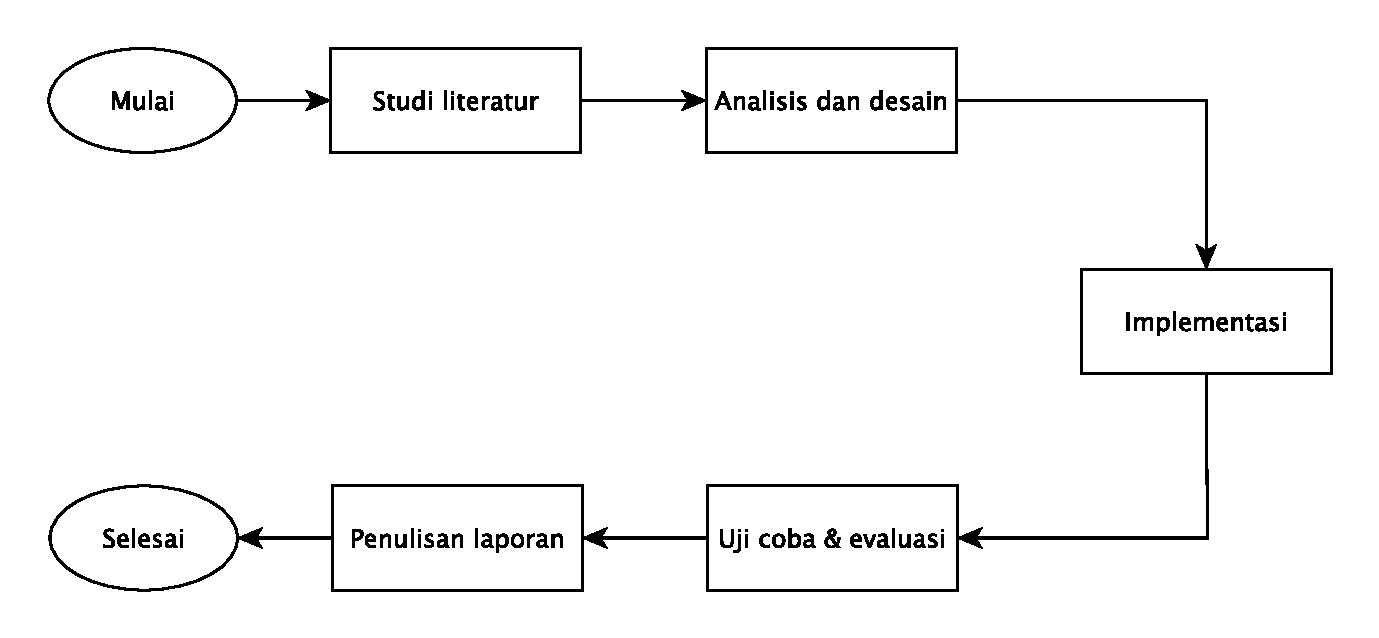
\includegraphics[scale=0.60]
  {images/3-tahapan}
\caption{Diagram Alir Tahapan Penelitian}
\label{fig:tahapan}
\end{figure}

\begin{enumerate}
  [noitemsep,
  nolistsep,
  leftmargin=0cm,
  itemindent=.5cm,
  listparindent=\parindent]

  \item Studi Literatur

    Dalam studi literatur, dikaji berbagai referensi mengenai konsep
    \tracking~dan arsitektur \pubsub~serta karakteristik \context~\aware. Dari
    hasil studi literatur ini, dapat ditemukan kekurangan dan kelebihan dari
    masing-masing topik. \Tracking~yang efisien harus bersifat adaptif dan
    efisien dikarenakan proses pembaharuan informasi yang bersifat sekuensial.
    Pada sistem \pubsub~mempunyai kelebihan yang dapat diadopsi pada proses
    \tracking, terutama dalam proses \tracking~multi target. Konsep ketertarikan
    konten digunakan untuk menjembatani proses \tracking~multi target.
    Karakteristik interaksi \pubsub, akan mengirimkan informasi melalui
    \event~\publish~ketika mendapatkan informasi yang baru. Hal ini perlu
    dilakukan penyesuaian sehingga didapatkan sistem \pubsub~yang efisien.

  \item Analisis dan Desain

    Tahap awal analisis dan desain adalah merumuskan kontribusi utama penelitian
    ini. Dari studi literatur yang telah dilakukan, dapat diketahui bahwa
    sistem \tracking~memerlukan mekanisme yang efisien dalam pembaharuan.
    Sistem \tracking~adaptif terhadap kebutuhan tingkat presisi suatu lokasi.
    Dalam tahap desain, dijelaskan langkah-langkah dalam proses pengerjaan
    penelitian. Rancangan dibagi dalam modul-modul sehingga mempermudah dalam
    tahap implementasi.

  \item Implementasi

    Pada tahap ini diimplementasikan rancangan sistem yang telah dibuat pada
    proses sebelumnya. Bahasa pemrograman yang digunakan adalah bahasa
    pemrograman Javascript dengan lingkungan pemrograman \nodejs. Implementasi
    menyangkut proses \content~\filtering berdasarkan
    \subscription~\language~yang telah dirancang. Dalam metode adaptif,
    dikembangkan juga modul mengenai \idle~\manager. Modul ini bertugas dalam
    penanganan proses \tracking~hanya pada informasi yang diperlukan.
    Implementasi ini dikembangkan dengan bantuan modul dari \nodejs, yaitu Mosca
    sebagai \middleware. Mosca mendukung protokol MQTT (MQ Telemetry Transport),
    sebuah protokol yang ringan dalam sistem \pubsub~sehingga cocok digunakan
    dalam komunikasi pada jaringan bergerak.

  \item Uji Coba dan Evaluasi

    Untuk menguji apakah kontribusi yang diajukan dapat berjalan dengan baik,
    maka diperlukan dilakukan suatu uji coba dengan berbagai macam skenario. Uji
    coba dilakukan dalam sebuah lingkungan \testbed~yang telah dipersiapkan.
    Skenario uji coba dilakukan dengan memberikan berbagai beban kerja dari
    berbagai parameter pada proses \tracking. Hasil uji coba dievaluasi untuk
    kemudian dianalisa sehingga dapat dilihat kinerja metode yang telah
    diajukan.

  \item Penulisan Laporan Penelitian

    Tahap ini adalah tahap untuk menyusun laporan penelitian. Setiap kegiatan
    yang dilakukan dalam penelitian didokumentasikan. Laporan berisi penjelasan
    mulai dari tahap studi literatur, analisa, tahap ujicoba serta kesimpulan
    dan saran.  Laporan penelitian ditulis sesuai dengan ketentuan yang berlaku.

\end{enumerate}

% }}} Tahapan Penelitian %

% Langkah-langkah Penelitian {{{ %
\section{Langkah-langkah Penelitian}

Langkah-Langkah penelitian secara umum disajikan dalam Gambar~\ref{fig:langkah}.
Langkah pertama adalah mempersiapkan lingkungan \testbed~yang digunakan dalam
evaluasi \pubsub. Selanjutnya, mempersiapkan data sampel yang digunakan dalam
proses \tracking.  Langkah selanjutnya adalah mengimplementasikan
\tracking~multi target, implementasi dilakukan pada sisi \client~serta~\server.
Kemudian, dilakukan uji coba dan evaluasi untuk mengetahui kinerja dari metode
yang diajukan pada lingkungan uji coba yang telah disiapkan dalam penelitian
ini.

\begin{figure}
  \centering
  \begin{tikzpicture}[font=\small, node distance=2cm, auto]
    \node[cloud] (start) {Mulai};
    \node[block, below of=start] (a) {Mempersiapkan lingkungan \pubsub};
    \node[block, below of=a] (b) {Mempersiapkan data sampel};
    \node[block, below of=b] (c) {Implementasi \tracking~multi target};
    \node[block, below of=c] (d) {Mempersiapkan lingkungan uji coba};
    \node[block, below of=d] (e) {Uji coba dan evaluasi};
    \node[cloud, below of=e] (end) {Selesai};

    \path[arrow] (start) -- (a);
    \path[arrow] (a) -- (b);
    \path[arrow] (b) -- (c);
    \path[arrow] (c) -- (d);
    \path[arrow] (d) -- (e);
    \path[arrow] (e) -- (end);
  \end{tikzpicture}
\caption{Langkah-langkah penelitian secara umum}
\label{fig:langkah}
\end{figure}

% Lingkungan PubSub {{{ %
\subsection{Lingkungan \PubSub}

Untuk mempersiapkan lingkungan \pubsub~diperlukan adanya suatu \middleware~pada
sisi \server~untuk menjembatani antara \publisher~dan \subscriber. Dalam
penelitian ini digunakan Mosca (http://github.com/mcollina/mosca). Tugas
\middleware~ini bertindak sebagai \broker, \middleware~ini dibangun menggunakan
bahasa pemrograman \nodejs.  Oleh karena itu sebelum konfigurasi Mosca
dilakukan, diperlukan pengaturan lingkungan \nodejs~pada sistem operasi.  Sistem
operasi yang dipilih adalah Debian GNU/Linux, dikarenakan kemudahan dalam
konfigurasi serta kehandalannya. Dalam lingkungan uji coba dibutuhkan IP publik
untuk \server. Dengan demikian server dapat diakses dari lingkungan bergerak
melalui jaringan operator 3G.

% }}} Lingkungan PubSub %

% Data Sampel {{{ %
\subsection{Data Sampel Uji Coba}

Sebelum melakukan uji coba dan evaluasi, dibutuhkan adanya data sampel uji coba.
Data sampel yang dibutuhkan berupa data lokasi \tracking~pada area kampus ITS
meliputi informasi \latitude~dan \longitude.  Untuk memudahkan mendapatkan data
sampel lokasi, digunakan proses pembangkitan lokasi. Dalam proses ini dibutuhkan
informasi mengenai jarak dua lokasi serta bearing, untuk kemudian ditentukan
lokasi berikutnya. Perhitungan jarak menggunakan persamaan \haversine, seperti
yang dijelaskan pada \equ~\ref{eq:haversine}

\noindent
\begin{equation}
	\label{eq:haversine}
	\begin{split}
	a = (\cos\varphi_2 \cdot \sin\bigtriangleup\lambda)^2
		+ (\cos\varphi_1 \cdot \sin\varphi_2
		- \sin\varphi_1 \cdot \cos\varphi_2 \cdot \cos\bigtriangleup\lambda)^2 \\
	b = \sin\varphi_1 \cdot \sin\varphi_2
		+ \cos\varphi_1 \cdot \cos\varphi_2 \cdot \cos \bigtriangleup\lambda \\
	c = atan2(\sqrt{a}, b) \\
	d = R \cdot c
	\end{split}
	\caption{Persamaan \Haversine}
\end{equation}

\begin{tabular}{l}
	Keterangan: \\
	R: Radius bumi \\
	\varphi: Latitude (dalam~radian) \\
	\lambda: Longitude (dalam~radian) \\
	d: Jarak dua lokasi \\
\end{tabular} \\

Persamaan \haversine~merupakan persamaan yang penting dan umum dipakai dalam
dunia navigasi, memberikan jarak lingkaran besar (\f{great circle}) antara dua
titik pada bumi berdasarkan \latitude~dan \longitude. Setiap area pada fokus
penelitian diambil nilai titik tengah (\centroid). Kedua nilai \centroid~inilah
yang diambil menjadi nilai masukkan pada proses pembangkitan. Nilai-nilai ini
disimpan dalam suatu berkas, dalam format JSON seperti yang dipaparkan pada
Gambar~\ref{fig:berkas_map}.

\noindent
\begin{figure}
	\centering
	\lstset{basicstyle=\ttfamily,frame=single,language=javascript}
	\lstinputlisting{src/map.json}
	\caption{Format Berkas Pembangkitan}
\label{fig:berkas_map}
\end{figure}

\noindent
\begin{equation}
	\label{eq:bearing}
	\begin{split}
		y = \sin(\bigtriangleup\lambda) \cdot \cos\varphi_2 \\
		x = \cos\varphi_1 \cdot \sin\varphi_2 - \sin\varphi_1 \cdot \cos\varphi_2
		\cdot \cos\bigtriangleup\lambda \\
		\theta = atan2(y, x)
	\end{split}
\end{equation}

\begin{tabular}{l}
	Keterangan: \\
	\varphi: Latitude (dalam~radian) \\
	\lambda: Longitude (dalam~radian) \\
	\theta: Bearing\\
\end{tabular}

\noindent
\begin{equation}
	\label{eq:destination}
	\begin{split}
		\varphi_2 = \arcsin(\sin\varphi_1 \cdot \cos(d/R) + \cos\varphi_1 \cdot
		\sin(d/R) \cdot \cos\theta) \\
		\lambda_2 = \lambda_1 + \arctan2(\sin\theta \cdot \sin(d/R) \cdot
		\cos\varphi_1, \cos(d/R) - \sin\varphi_1 \cdot \sin\varphi_2)
	\end{split}
\end{equation}

\begin{tabular}{l}
	Keterangan: \\
	R: Radius bumi \\
	d: Jarak perpindahan \\
	\varphi: Latitude (dalam radian) \\
	\lambda: Longitude (dalam radian) \\
	\theta: Bearing\\
\end{tabular} \\

Dari \equ~\ref{eq:haversine}, \equ~\ref{eq:bearing} serta
\equ~\ref{eq:destination} menjadi masukkan dalam proses pembangkitan data
lokasi. Proses lebih jelas dijabarkan pada Gambar~\ref{fig:pembangkitan}. Proses
pembangkitan dimulai dengan menentukan \centroid~lokasi awal dan
\centroid~lokasi tujuan. Dari kedua nilai \centroid, kemudian dicari jarak
antara dua titik menggunakan ~\ref{eq:haversine} (Haversine). Untuk mencari
lokasi tujuan berikutnya, dibutuhkan juga nilai \bearing. Proses pencarian
lokasi tujuan akan dilakukan sampai jarak dua lokasi tercapai. Nilai jarak awal
diakumulasi mengikuti kecepatan perpindahan obyek \tracking.  Kecepatan
perpindahan obyek diasumsikan sebesar 1.4 m/s, kecepatan berjalan manusia.

\noindent
\begin{figure}
	\centering
	\lstset{basicstyle=\ttfamily,frame=single}
	\lstinputlisting{src/generator.pseudo}
	\caption{Pseudocode Langkah Pembangkitan Lokasi}
\label{fig:pembangkitan}
\end{figure}

Data-data lokasi yang telah dibangkitkan pada proses pembangkitan, kemudian akan
disimpan dalam sebuah berkas berformat JSON (\f{Javascript Object Notation})
Array. Format dapat dilihat pada Gambar~\ref{fig:pembangkitan_data}. Berkas ini
digunakan sebagai nilai masukkan \publisher~pada lingkungan \testbed~yang telah
disiapkan. Terdapat tiga elemen penting dalam setiap informasi lokasi, yaitu: id
(id lokasi informasi), lat (\latitude~lokasi) dan lng (\longitude~lokasi).
Informasi-informasi lokasi ini disimpan dalam array satu dimensi. Setiap
informasi lokasi sebelum di-\publish~akan disisipi informasi waktu yang
digunakan untuk proses evaluasi dalam format \unixtimetstamp(\miliseconds).

Data-data informasi lokasi ini merepresentasikan pergerakan \publisher~dalam
lingkungan \testbed. \Publisher~akan membaca setiap informasi lokasi dalam
format JSON, untuk kemudian disimulasikan proses \publish~informasi ke \broker.
Simulasi pengiriman akan dilakukan dalam kurun waktu tertentu. Simulasi ini
selain dipengaruhi oleh waktu, dipengaruhi juga oleh ketertarikan konten
informasi lokasi secara adaptif pada \subscriber. Pada metode adaptif hanya akan
dilakukan proses \publish~untuk informasi lokasi yang dibutuhkan oleh
\subscriber.

\noindent
\begin{figure}
	\centering
	\lstset{basicstyle=\ttfamily,frame=single,language=javascript}
	\lstinputlisting{src/pembangkitan-data.json}
	\caption{Contoh Data Proses Pembangkitan}
\label{fig:pembangkitan_data}
\end{figure}

% }}} Data Sampel %

% Implementasi {{{ %
\subsection{Implementasi}

Pada penelitian sebelumnya (Kjaergaard dkk, 2009) telah diimplementasikan sistem
\tracking~yang efisien untuk perangkat bergerak. Sayangnya sistem \tracking~ini
kurang mengakomodir untuk proses \tracking~multi target. Sistem \pubsub~ideal
pada lingkungan jaringan tak handal seperti WSN (Hunkeler dkk, 2008). Karena
karakter lingkungan WSN yang hampir sama dengan jaringan bergerak, sehingga hal
ini dapat diadopsi.

% fig:sistem {{{ %
\noindent
\begin{figure}
  \centering
  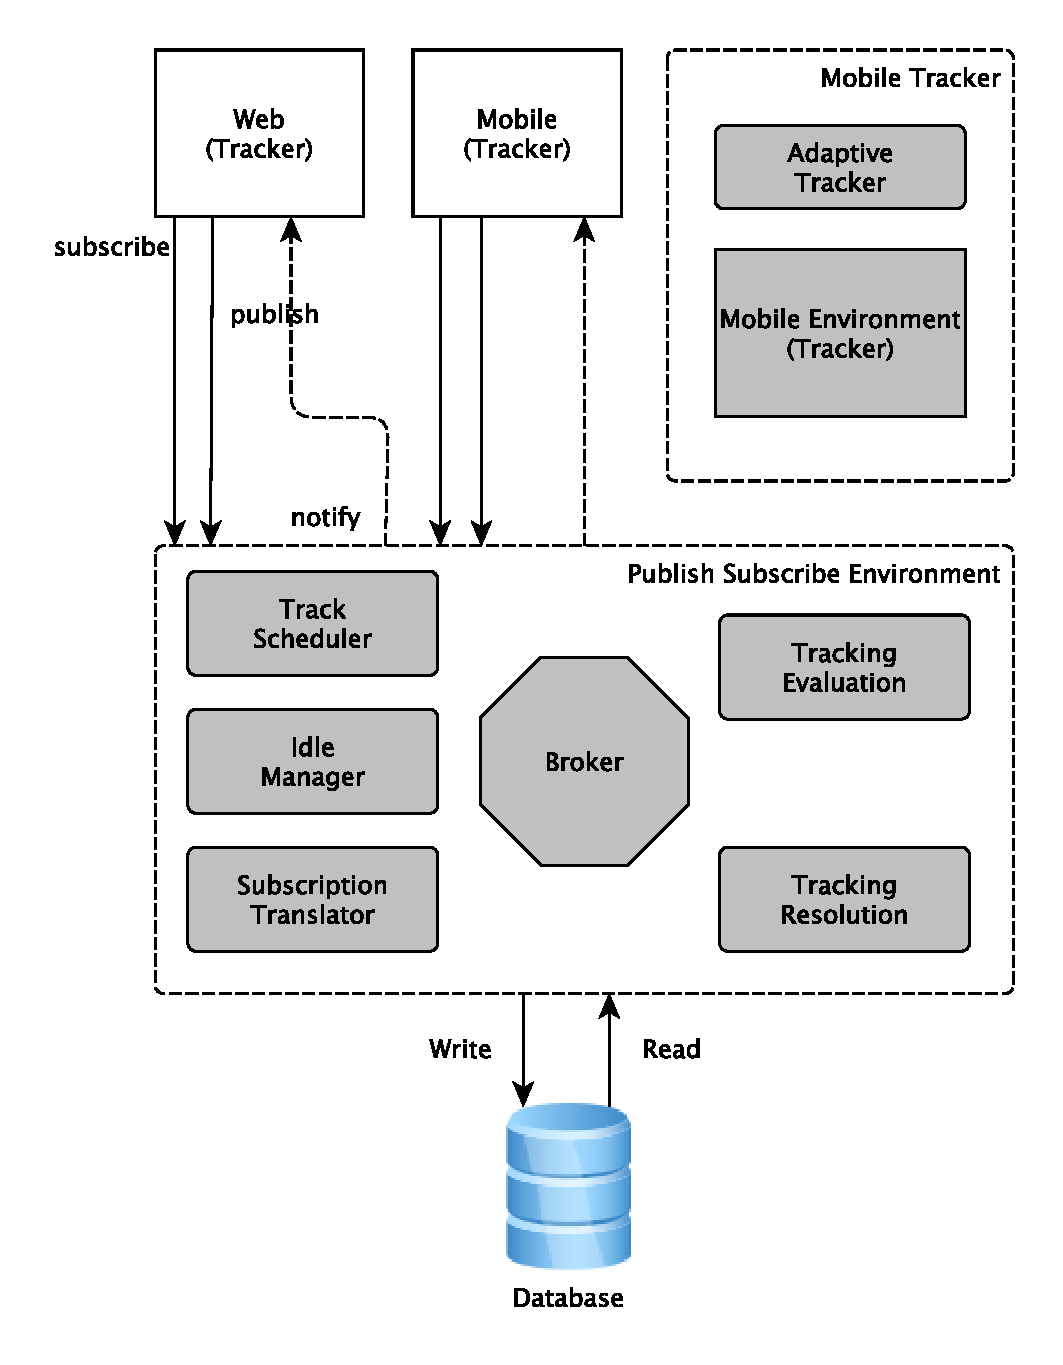
\includegraphics[scale=0.60]
  {images/3-sistem}
  \caption{Arsitektur rancangan sistem}
\label{fig:sistem}
\end{figure}
% }}} fig:sistem %

Interaksi antara \publisher~(entitas yang menjadi target \tracking) dengan
\subscriber~(entitas yang melakukan \tracking~atau \f{tracker}) dapat dipaparkan
pada Gambar~\ref{fig:sistem}.  \Publisher~akan mengirimkan \event~kepada sistem
\pubsub~berupa informasi \tracking.  Sedangkan \subscriber~mengirimkan
\subscription~yang diatur dalam \f{subscription language} kepada sistem \pubsub,
\subscriber~hanya akan dinotifikasi sesuai dengan ketertarikannya melalui proses
\f{tracking evaluation}. \Subscription~yang ada akan diterjemahkan oleh
\f{subscription translator}. Notifikasi ke entitas \subscriber, akan ditangani
oleh \broker. Entitas \subscriber~dapat berwujud \f{mobile client} maupun \f{web
  client}. Pada metode adaptif, terdapat \f{idle manager} yang mengatur
\publisher~untuk melakukan \event~\publish~ke \broker~atau tidak.
\Publisher~hanya akan aktif melakukan \event~\publish~apabila informasi lokasi
yang di-\publish~dibutuhkan oleh \subscriber.

% Dalam perangkat bergerak, ditanamkan sebuah modul adaptif dalam penentuan
% lokasi.  Modul ini akan mendeteksi aktifitas obyek yang diamati, dari aktifitas
% pini menjadi dasar klasifikasi kebutuhan pembaruan serta presisi lokasi. Deteksi
% aktifitas didasarkan pada data \f{sampling} yang direkam menggunakan sensor
% \acc.

\noindent
\begin{figure}
  \centering
  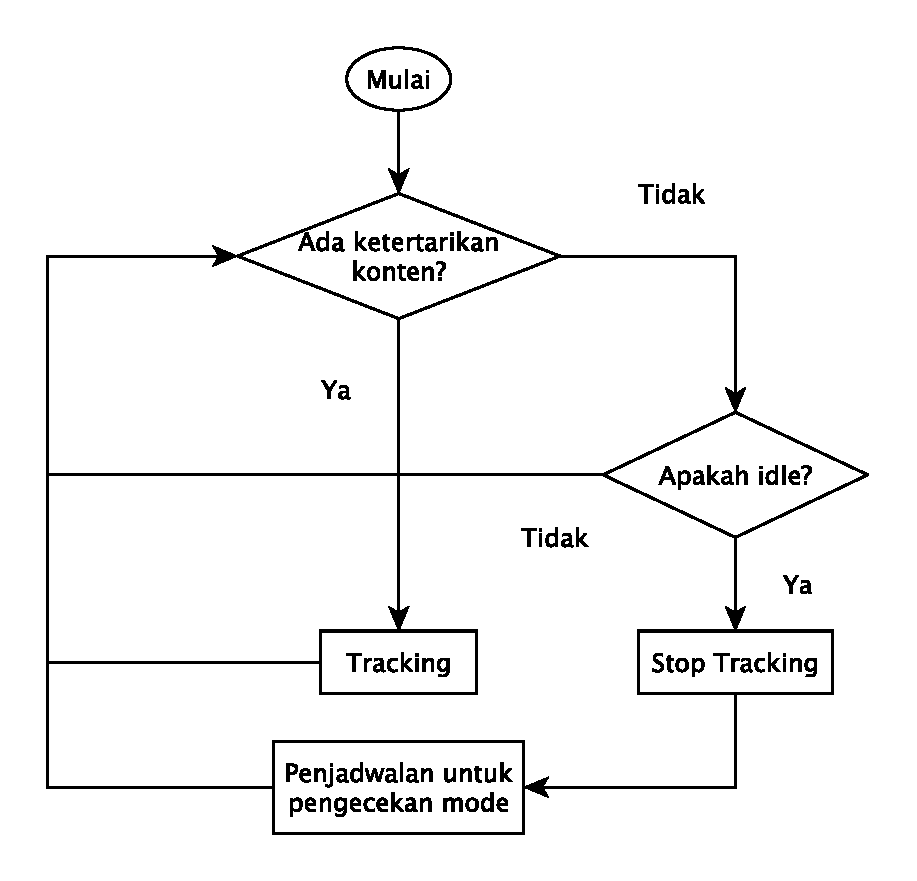
\includegraphics[scale=0.70]
  {images/3-adaptive-tracking}
  \caption{Diagram Alir Metode Adaptif}
\label{fig:adaptive_tracking}
\end{figure}

Karakteristik interaksi pada sistem \pubsub~tradisional, walaupun informasi dari
\publisher~tidak dibutuhkan, pihak \publisher~akan tetap melakukan
\event~\publish~informasi ke \broker. Untuk mengurangi hal ini, diperlukan
mekanisme untuk menangani masalah ini seperti terlampir pada
Gambar~\ref{fig:adaptive_tracking}. Mekanisme ini diimplementasikan pada sisi
\server. Dalam komunikasi data pada proses \tracking~akan diadopsi dengan skema
\pubsub~dengan protokol MQTT (MQ Telemetry Transport).

% NodeJS {{{ %
\section{Pemrograman \nodejs}

\nodejs~adalah sebuah platform baru yang menarik untuk pengembangan aplikasi
web, server, maupun kebutuhan jaringan \server~atau \client serta pemrograman
yang umum. Platform ini didesain untuk skalabilitas dalam aplikasi jaringan
dengan menggabungkan bahasa Javascript pada sisi \server, \asynchronous I/O dan
pemrograman asynchronous. Arsitektur platform ini berbasis \event-\driven~dengan
\f{single-threading}.

Pemrograman \nodejs~sangat berbeda dengan pemrograman aplikasi server pada
umumnya yang skalabilitasnya menggunakan \thread. \nodejs~diklaim mempunyai
kebutuhan memori rendah, tinggi \throughput, \latency~lebih baik dengan model
pemrograman yang sederhana. Platform \nodejs~dalam fase perkembangan yang cukup
cepat, selain itu juga cukup menjanjikan sebagai alternatif dari Java, PHP,
Python, Ruby.

Platform \nodejs~diimplementasikan dengan non-blocking I/O event loop dan
pustaka network I/O, dibangun di atas V8 Javascript engine (dari Chrome web
browser). Pustaka I/O mampu mengimplementasikan protokol TCP atau UDP pada
server, seperti DNS, HTTP, IRC ataupun FTP\@. Kebanyakan penggunaan platform ini
pada aplikasi \realtime, sebagai contoh monitoring dengan pustaka Socket.IO.

Pada Gambar~\ref{fig:nodejs} merupakan contoh sederhana pemrograman \nodejs.
Pemrograman tersebut memanfaatkan modul http pada \nodejs~untuk membangun sebuah
web server sederhana yang berjalan pada port 1337. Ketika dibuka pada browser,
fungsi anonymous akan menangkap \request~dan menampilkan \response~dengan kode
http 200, bertuliskan Hello World.

\noindent
\begin{figure}
	\centering
	\lstset{basicstyle=\ttfamily,frame=single,language=javascript}
	\lstinputlisting{src/node.js}
	\caption{Contoh Pemrograman \nodejs}
	\label{fig:nodejs}
\end{figure}

% Modul NodeJS {{{ %
\subsection{Modul \nodejs}

Dalam pemrograman \nodejs~sangat tergantung dengan modul, modul adalah blok
dasar dalam membangun aplikasi \nodejs. Sebuah modul mengenkapsulasi
fungsi, menyembunyikan detil dalam sebuah kontainer. Setiap modul dapat
mempunyai ketergantungan dengan modul yang lain. Informasi ini disimpan dalam
sebuah berkas package.json. Pada Gambar~\ref{fig:package_json} dipaparkan mengenai
format dasar mengenai ini. Berkas tersebut berisi informasi mengenai nama modul,
versi serta daftar ketergantungan modul-modul yang disimpan dalam format JSON.

\noindent
\begin{figure}
	\centering
	\lstset{basicstyle=\ttfamily,frame=single,language=javascript}
	\lstinputlisting{src/package.json}
	\caption{Contoh Berkas package.json}
	\label{fig:package_json}
\end{figure}

Untuk mengatur modul-modul \nodejs, digunakan perkakas npm (\f{node package
	management}). Perkakas ini menjadi standar dalam mengatur dan mendistribusikan
modul untuk \nodejs. Secara konseptual perkakas ini serupa dengan apt-get
(Debian), rpm/yum (Red Hat/Fedora), Homebrew (Mac OS X), CPAN (Perl) atau
Composer (PHP). Ditujukan untuk digunakan mem-\publish~dan mendistribusikan
modul node dalam internet menggunakan antarmuka perintah sederhana, melakukan
instalasi dan mengatur modul yang telah terinstal.

Dalam penelitian ini memanfaatkan beberapa modul \nodejs~untuk memudahkan proses
pengembangan. Modul-modul tersebut antara lain:

\begin{enumerate}[noitemsep, nolistsep]
    \item Mosca (http://github.com/mcollina/mosca)
			Mosca adalah sebuah MQTT broker yang dapat digunakan secara \f{standalone}
			atau ditanam dalam aplikasi \nodejs.
    \item Express (http://expressjs.com)
      Express adalah framework aplikasi untuk platform \nodejs~yang fleksibel
      serta menyediakan fitur yang \robust~untuk aplikasi web dan \f{mobile}.
    \item Async (http://github.com/caolan/async)
			Async adalah sebuah modul utilitas yang menyediakan fungsi untuk menangani
			asynchronous Javascript.
    \item Bunyan (http://github.com/trentm/node-bunyan)
			Sebuah modul sederhana yang handal yang menyediakan fitur \f{logging}
			dalam format JSON.
		\item Node-MySql (http://github.com/felixge/node-mysql)
			Implementasi protokol klien MySql dengan pemrograman \nodejs.
		\item Node-Usage (http://github.com/arunoda/node-usage)
			Modul antar muka untuk mengakses penggunaan CPU dan RAM, terbatas pada
			lingkungan UNIX.
		\item Node-Schedule (http://github.com/tejasmanohar/node-schedule)
			Modul untuk \scheduler~dengan format cron-like maupun not-cron-like.
\end{enumerate}

% }}} Modul NodeJS %

% Mosca {{{ %
\subsection{Modul Mosca}

Mosca merupakan modul \broker~yang dapat ditanam dalam aplikasi \nodejs. Modul
ini dikembangkan oleh pengembang dari Italia yang tertarik dengan dunia IoT
(\f{Internet of Things}), yaitu Matteo Collina. Komunikasi pada \broker~dibangun
dengan menggunakan protokol MQTT. Untuk skalabilitas, \broker~ini mendukung
clustering dengan bantuan dari \broker~lain. Diantara \broker~yang didukung,
antara lain:

\begin{enumerate}[noitemsep, nolistsep]
    \item Redis, sebuah basis data nosql berorientasi key/value yang dibuat oleh
			Salvatore Sanfilippo.
    \item MongoDB, basis data berorientasi dokumen dengan performa tinggi.
    \item Mosquitto (protokol MQTT)
		\item RabbitMQ (protokol AMQP)
		\item ZeroMQ
\end{enumerate}

Selain performa skalabilitas dengan dukungan dari \broker~lain, didapatkan juga
dukungan beberapa protokol seperti AMQP serta MQTT. Mosca juga mendukung
websocket sehingga dapat diaplikasikan dalam aplikasi realtime pada platform
web. Dukungan websocket didapatkan dengan menggunakan \f{MQTT over websocket}
yang di-\f{bundle} dengan browserify. Dengan adanya dukungan ini, modul Mosca
dapat dikolaborasikan dengan modul Express.

Protokol MQTT pada Mosca menggunakan MQTT.js. Modul ini yang menangani interaksi
antara \client~dan \broker. MQTT.js mendukung (\f{Quality of Service}) QoS 0,
Qos 1 dan QoS 2. Dukungan QoS tergantung dari \broker~yang digunakan. Untuk saat
ini tidak semua \broker~mendukung semua QoS. Modul ini menangani beberapa proses
yang umum dalam lingkungan \pubsub, seperti \f{connect}(), \f{publish}(),
\f{subscribe}(), \f{unsubscribe}(), \f{close}().

Seperti pada umumnya pemrograman \nodejs~yang berbasis \event, dalam Mosca
terdapat \event~yang dapat digunakan untuk memperdalam fungsionalitas. Event
\ready, \clientConnected, \published, \subscribed dan \clientDisconnected. Pada
\event~\clientConnected~digunakan untuk mendeteksi adanya \client~yang sedang
terhubung dengan sistem \pubsub. Sedangkan pada \clientDisconnected~untuk
mendeteksi \client~yang keluar. Pada event \published~serta \subscribed~dapat
digunakan untuk melakukan evaluasi konten yang keluar-masuk dalam sistem \pubsub.
Pada Gambar~\ref{fig:mosca} ditunjukkan mengenai contoh penggunaan modul ini.

\noindent
\begin{figure}
	\centering
	\lstset{basicstyle=\footnotesize\ttfamily,frame=single,language=javascript}
	\lstinputlisting{src/mosca.js}
	\caption{Contoh Penggunaan Modul Mosca}
	\label{fig:mosca}
\end{figure}

% }}} Mosca %

% Modul Async {{{ %
\subsection{Modul Async}

Async adalah sebuah modul utilitas yang menyediakan fungsi untuk menangani
asynchronous Javascript. Modul ini menyediakan sekitar 20 fungsi yang secara
umum digunakan dalam mengelola alur kontrol \asynchronous. Platform
\nodejs~menggunakan \event~\driven~dengan \thread~tunggal yang berjalan secara
\asynchronous, hal ini sangat berbeda dengan platform pemrograman yang lain.
Modul ini sangat membantu dalam mengelola urutan eksekusi fungsi \anonymous~pada
\nodejs.

\noindent
\begin{figure}
	\centering
	\lstset{basicstyle=\footnotesize\ttfamily,frame=single,language=javascript}
	\lstinputlisting{src/series.js}
	\caption{Contoh Penggunaan Alur Kontrol \series}
\label{fig:async_series}
\end{figure}

Dalam penelitian ini hanya digunakan alur kontrol, \series~serta \waterfall.
Alur kontrol \series~menjamin eksekusi fungsi \anonymous~dilakukan secara
berurutan. Contoh penggunaan alur kontrol ini dapat dilihat pada
Gambar~\ref{fig:async_series}. Sedangkan alur kontrol \waterfall, hasil eksekusi
fungsi \anonymous~akan menjadi masukan fungsi \anonymous~berikutnya. Contoh
penggunaan alur kontrol ini dapat dilihat pada Gambar~\ref{fig:async_waterfall}.

\noindent
\begin{figure}
	\centering
	\lstset{basicstyle=\footnotesize\ttfamily,frame=single,language=javascript}
	\lstinputlisting{src/waterfall.js}
	\caption{Contoh Penggunaan Alur Kontrol \waterfall}
\label{fig:async_waterfall}
\end{figure}

Alur kontrol ini sangat berguna dalam proses evaluasi konten yang
di~\publish~oleh \publisher. Setiap konten perlu dilakukan proses pencocokan
sesuai dengan ketertarikan \subscriber~dengan konten dari \publisher. Alur
kontrol \series~digunakan dalam mengatur proses pencocokan kumpulan ketertarikan
untuk masing-masing \subscriber. Sedangkan alur kontrol \waterfall~digunakan
dalam menangani hasil pencocokan \subscriber~satu dengan \subscriber~lainnya.
Alur kontrol \waterfall~memastikan konten yang di-\publish~masih dibutuhkan
dalam proses \tracking.

% }}} Modul Async %

% }}} NodeJS %

% }}} Implementasi %

% Location Model {{{ %
\section{\f{Location Model} dan \f{Tracking Resolution}}

Pada proses komunikasi antara \f{tracker} dengan obyek yang menjadi target
\tracking~terjadi adanya pertukaran data. Dengan ini diperlukan pemodelan data
yang dikirimkan. Dalam Tabel~\ref{tab:model} dipaparkan pemodelan data yang
dimaksud. Setiap target \tracking~mempunyai atribut id, code, user, lat, lng
dan time. Deskripsi setiap atribut dijelaskan pada kolom Keterangan.

Atribut lat, lng dan time didapatkan dari proses pembangkitan data pada data
sampel uji coba. Sedangkan atribut code, action serta user dikirimkan oleh
\broker~kepada \subscriber. Atribut code, merepresentasikan apakah status
informasi yang diperoleh (OK atau ERR). Atribut user, merepresentasikan
kepemilikan obyek informasi lokasi yang didapatkan. Sedangkan atribut action,
merepresentasikan respon yang diterima. Atribut ini juga yang mengatur perlu
tidaknya dilakukan proses \event~\publish~pada \publisher.

\begin{table}
\centering
\caption{Data Model}
\label{tab:model}
  \begin{tabular}{l l l}
    \hline
    Atribut & Tipe           & Keterangan                               \\
    \hline
		id			& Integer				 & \f{Identifier}		\\
    code    & String         & Protokol status respon (OK atau ERR) \\
    action  & string         & Protokol aksi respon yang diterima \\
    user    & String         & Nama dari obyek yang di-\f{track}        \\
    lat     & Double         & Nilai \latitude                          \\
    lng     & Double         & Nilai \longitude                         \\
    time    & Unix Timestamp & Informasi mengenai waktu data dikirimkan \\
    \hline
  \end{tabular}
\end{table}

\f{Tracking resolution} membagi kedalaman tingkat informasi menjadi beberapa
resolusi, pada Gambar~\ref{fig:tracking-resolution} dan
Tabel~\ref{tab:tracking-resolution} ditunjukkan mengenai pemodelan resolusi
serta contoh informasi yang didapatkan.  Setiap resolusi merepresentasikan level
hak akses, semakin kecil level hak akses, maka tingkat kedalaman informasi akan
semakin detil. Contoh: pada level 3, \f{tracker} hanya dapat memperoleh
informasi resolusi Zona, tetapi pada level 1 \f{tracked} memperoleh informasi
sampai koordinat yang berupa longitude dan latitude.

% img:tracking-resolution {{{ %
\begin{figure}
    \centering
    \includegraphics[scale=0.80]
    {images/3-tracking-resolution.png}
    \caption{Pembagian Tingkat \f{Tracking Resolution}}
\label{fig:tracking-resolution}
\end{figure}
% }}} img:tracking-resolution %

Pada penelitian ini pembagian level hak akses dibatasi hanya sampai dengan empat
level. Level pertama mewakili koordinat \latitude~dan \longitude. Untuk level
kedua merepresentasikan nama Gedung. Level hak selanjutnya mewakili nama Zona.
Dan level hak akses terakhir mewakili Area, yaitu kampus ITS. Untuk setiap nama,
diwakili oleh \centroid~\latitude~dan \longitude~berdasarkan pembagian resolusi
informasi lokasi.

% tab:tracking-resolution {{{ %
\begin{table}
\centering
\caption{Contoh Data \f{Tracking Resolution}}
\label{tab:tracking-resolution}
    \begin{tabular}{l l l}
        \hline
        Level & Resolusi & Data \\
        \hline
        Level 1 & Koordinat & Lon: 123,456 Lat: -123,456 \\
        Level 2 & Gedung & Gedung Teknik Informatika, Gedung Rektorat \\
        Level 3 & Zona & Zona Barat, Zona Timur \\
        Level 4 & Area & ITS, Luar ITS \\
        \hline
    \end{tabular}
\end{table}
% }}} tab:tracking-resolution %

Pemodelan lokasi yang digunakan merupakan gabungan antara \f{Geometric} dan
\f{Symbolic} yang bersifat hirarkis. Resolusi suatu informasi lokasi dipengaruhi
oleh level hak akses, \tracker~yang mempunyai \Role~lebih tinggi atau selevel
dengan target \tracking~memiliki resolusi informasi yang lebih detil.  Pada
Gambar~\ref{fig:tracking-resolution} lingkungan Kampus Institut Teknologi
Sepuluh Nopember (ITS) dibagi menjadi empat tingkat level. Seorang \tracker~yang
mempunyai hak akses level 4 hanya dapat mengetahui informasi sebatas target
\tracking~sedang berada di wilayah kampus ITS atau tidak. Sedangkan untuk
\tracker~yang mempunyai hak akses lebih tinggi dapat memperoleh informasi sampai
level gedung/bangunan sampai koordinat.

% img:location-hierarchy {{{ %
\begin{figure}
    \centering
    \includegraphics[scale=0.60]
    {images/3-location-hierarchy.png}
    \caption{Location Model secara hirarkis}
\label{fig:location-hierarchy}
\end{figure}
% }}} img:location-hierarchy %

% }}} Location Model %
% Subscription Language Translator {{{ %

\section{\f{Subscription Language Translator}}

Seorang \f{tracker} agar dapat melakukan proses \f{tracking} diperlukan untuk
berkomunikasi menggunakan aturan-aturan yang telah disepakati. \f{Tracker} dapat
melakukan \f{tracking} dengan berbagai kriteria, seperti \f{channel}, area, zona
serta jarak dan waktu. Pesan yang dikirimkan ke \f{broker} akan ditranslasi oleh
modul \f{subscription language translator}. Kriteria-kriteria di atas dapat
dilakukan operasi matematika logika antara kriteria satu dengan kriteria
lainnya.

Dari proses translasi oleh modul pada \broker, akan dikembalikan kepada
\f{tracker} kembali untuk dijadikan sebagai protokol \f{subscription}. Format
protokol ini merupakan gabungan antara satu kriteria atau lebih, dalam bentuk
\f{expression boolean}. Dalam protokol ini berlaku operasi-operasi sesuai dengan
Tabel\ref{tab:operator-comparison} dan Tabel\ref{tab:operator-logical}. Contoh:
area = 'ITS', area = 'FTIF' and user = 'publisher1'.

% tab:operator-comparison {{{ %
\begin{table}
\centering
\caption{Operator perbandingan}
\label{tab:operator-comparison}
\begin{tabular}{l l}
  \hline
  Operator & Keterangan \\
  \hline
  = & Operator sama dengan \\
  <> & Operator tidak sama dengan \\
  \textgreater{} & Operator lebih besar \\
  \textless{} & Operator lebih kecil \\
  \textgreater{}= & Operator lebih besar sama dengan \\
  \textless{}= & Operator lebih kecil sama dengan \\
  \hline
\end{tabular}
\end{table}
% }}} img:operator-comparison %

% tab:operator-logical {{{ %
\begin{table}
\centering
\caption{Operator logika}
\label{tab:operator-logical}
\begin{tabular}{l l}
    \hline
    Operator & Keterangan \\
    \hline
    and & Operator AND \\
    or & Operator OR \\
    \hline
\end{tabular}
\end{table}
% }}} img:operator-logical %

% }}} Subscription Language Translator %

% }}} Langkah-langkah Penelitian %

% Uji Coba dan Evaluasi {{{ %
\section{Uji Coba dan Evaluasi} Untuk mengetahui efisiensi serta kevalidan
penelitian berdasarkan sistem yang dirancang, perlu dilakukan uji coba dan
evaluasi. Pada bagian ini dipaparkan mengenai tahapan uji coba serta evaluasi
yang dilakukan. Tahapan-tahapan itu meliputi, skenario, lingkungan serta
parameter-parameter uji coba yang dilakukan. Dari hasil yang diperoleh,
dilakukan tahapan evaluasi.

% Skenario Uji Coba {{{ %
\subsection{Skenario Uji Coba}

Uji coba yang dilakukan menguji dua metode interaksi, yaitu: metode adaptif yang
diusulkan dan sebagai pembanding digunakan model interaksi sistem
\pubsub~tradisional (non-adaptif). Uji coba dilakukan pada lingkungan
\testbed~yang telah dibangun. Pada sisi \server, terdapat suatu \broker~yang
menjembatani proses \tracking~antara \publisher~dan \subscriber. Uji coba
dilakukan dengan mesimulasikan data sampel dalam lingkungan \testbed~selama 5
menit dengan jumlah \publisher~dan~\subscriber yang bervariasi. Pada proses ini
dilakukan evaluasi parameter-parameter uji coba, meliputi CPU \server, RAM
\server, \bandwidth~serta \latency. Jaringan yang digunakan adalah jaringan 3G
dan jaringan Wi-Fi.

% }}} Skenario Uji Coba %

% Lingkungan Uji Coba {{{ %
\subsection{Lingkungan Uji Coba}

Pada sistem \tracking~multi target ini terdapat dua komponen utama,
yaitu \client~dan \server. \Client~merupakan entitas yang menjadi target
\tracking~atau yang melakukan \tracking~(bertindak sebagai \publisher~atau
\subscriber). Pada sisi \server~terdapat sebuah sistem \pubsub~tunggal, yang
memiliki IP publik. Sistem \pubsub~dibangun menggunakan Mosca sebagai
\broker, dan untuk protokol komunikasi dengan \client~menggunakan protokol
MQTT\@.

\begin{figure}
  \centering
  \includegraphics[scale=0.4]
	{images/3-its.png}
  \caption{Denah lokasi kampus Institut Teknologi Sepuluh Nopember}
\label{fig:its}
\end{figure}

Area \tracking~yang digunakan adalah area kampus Insitut Teknologi Sepuluh
Nopember (Gambar~\ref{fig:its}) yang sudah dilakukan pemodelan lokasi.
Pembatasan area ini untuk memudahkan pengujian dan analisa. Proses
\tracking~dilakukan pada orang yang bergerak dengan berjalan kaki (pedestrian)
tanpa bantuan kendaraan yang disimulasikan dengan data sampel.

% Deteksi CPU & RAM {{{ %
\subsection{Deteksi Sumber Daya CPU dan RAM}

Deteksi sumber daya CPU dan RAM dilakukan dengan mencatat penggunaan sumber daya
oleh suatu PID (\f{Process ID}) yang dibaca ke dalam suatu log dalam interval
waktu tertentu. Untuk memudahkan proses ini digunakan modul \f{node-usage}
(http://github.com/arunoda/node-usage). Pada Gambar~\ref{fig:usage} dan
Gambar~\ref{fig:usage_result} dijabarkan penggunaan modul ini. Proses ini akan
diulang sejumlah perubahan banyaknya \publisher~dan \subscriber~untuk setiap
metode, baik adaptif maupun non adaptif. Proses ini dilakukan pada sisi \server.

\noindent
\begin{figure}
	\centering
	\lstset{basicstyle=\ttfamily,frame=single,language=javascript}
	\lstinputlisting{src/usage.js}
	\caption{Contoh Penggunaan Modul node-usage}
\label{fig:usage}
\end{figure}


\noindent
\begin{figure}
	\centering
	\lstset{basicstyle=\ttfamily,frame=single,language=javascript}
	\lstinputlisting{src/result-object.js}
	\caption{Informasi Data Penggunaan Sumber Daya}
\label{fig:usage_result}
\end{figure}
% }}} Deteksi CPU & RAM %

% Estimasi \Bandwidth {{{ %
\subsection{Estimasi \Bandwidth}

Pada evaluasi \bandwidth, digunakan \f{dumpcap} (perkakas \f{tcpdump} pada
Wireshark). Dikarenakan lingkungan Unix tidak mendukung proses \f{Remote Packet
	Capture}, proses ini akan dilakukan dengan bantuan \f{SSH tunnel} sebagai
alternatif \f{Remote Capture Interface}. Proses evaluasi akan dilakukan dengan
menggunakan jaringan 3G dan Wi-Fi.

% }}} Estimasi \Bandwidth %

% Estimasi Latency {{{ %
\subsection{Estimasi Latency}

Estimasi latency dilakukan dengan menggunakan pencatatan dalam log, informasi
waktu yang dibutuhkan pada paket yang di\publish~oleh \publisher~untuk sampai
kepada~\subscriber. Proses pencatatan ini dilakukan untuk kedua metode, baik
adaptif maupun non adaptif. Dikarenakan pada metode adaptif tidak semua data
sampel dikirimkan, maka pada proses evaluasi akan dilakukan pemilahan log.
Pemilahan log didasarkan pada informasi id serta \publisher.
% }}} Estimasi Latency %

% }}} Lingkungan Uji Coba %

% Data Uji Coba {{{ %
\subsection{Data Uji Coba}

Dalam evaluasi uji coba digunakan data lokasi yang dibangkitkan menggunakan
gabungan persamaan antara \bearing~dan jarak dua lokasi area (diambil nilai
\centroid~dari masing-masing lokasi). Dari dua lokasi yang diketahui akan dicari
nilai \bearing~untuk kemudian digunakan sebagai acuan dalam penentuan pergeseran
posisi lokasi berikutnya. Besarnya pergeseran posisi lokasi diasumsikan
menggunakan kecepatan berjalan manusia yaitu 1.4 m/s.

Data yang telah dibangkitkan kemudian disimpan dalam sebuah berkas dengan format
JSON (Javascript Object Notation). Berkas-berkas data menjadi nilai masukkan
dalam proses evaluasi pada \testbed~yang telah dipersiapkan.

% }}} Data Uji Coba %

% }}} Uji Coba dan Evaluasi %
